\chapter{Preliminaries}

%123456789 123456789 123456789 123456789 123456789 123456789 123456789 123456789

In this chapter we provide an overview of the elementary concepts we use
throughout the thesis.

\section{Notion}

We briefly summarize the notion we use. We use standard notion for number
systems: $\mathbb{N}$ for natural numbers (including zero), $\mathbb{R}$ for
real numbers, $\mathbb{R}^+$ for positive real numbers and $\mathbb{R}^+_0$
for non-negative real numbers.

We shall often work with vectors, we shall write them as $\vec{a}$. In order
to refer to $i$-th element of a vector $\vec{a}$ we shall write $a_i$.
Similarly, in case of matrix $A$, we shall refer to specific element as
$A_{i,j}$ in $i$-th row and in $j$-th column.

Finally, we shall use the term \emph{tensor} as a generalization of vectors
and matrices. We shall use following recursive definition

\begin{defn}
0-dimensional tensor is a single number. n-dimensional ($n > 0$) vector of sizes
$(s_1, s_2, \ldots, s_n)$ is an ordered set of $s_1$ $(n-1)$-dimensional
tensors of sizes $(s_2, s_3, \ldots, s_n)$.
\end{defn}

As we can see, 1-dimensional tensor is a vector and 2-dimensional tensor is
a matrix. Similarly, we shall refer to specific element of tensor $a$ using
subscripts ($a_{i,j,k}$).

\section{Distance and Metric Spaces}
\label{sec:distances}

In this work we often need to express similarity between two datapoints
(usually images or their representation). To provide a precise mathematical
background for such similarity we use the concept of metric spaces introduced
by \cite{metric} and named by \cite{metricname}. We further differentiate
between metrics (and metric spaces) and distances (and distance spaces). We
use definitions per \cite{deza2009encyclopedia}.

\begin{defn}
Metric space $(\mathcal{F}, \delta)$ is a pair of set $\mathcal{F}$ and
corresponding distance function
$\delta : \mathcal{F} \times \mathcal{F} \goto \mathbb{R}_0^+$ such that
following axioms hold:
\begin{itemize}
    \item $\delta(x, y) = 0 \Leftrightarrow x = y$ (Coincidence axiom)
    \item $\delta(x, y) = \delta(y, x)$ (Axiom of symmetry)
    \item $\delta(x, y) \leq \delta(x, z) + \delta(z, y)$ (Triangle inequality)
\end{itemize}
\end{defn}%

However, as these axioms prove to be too restrictive in some cases, we also
use the concept of distance space:
\begin{defn}
Distance space $(\mathcal{F}, \delta)$ is a pair of set $\mathcal{F}$ and
corresponding distance function $\delta : \mathcal{F} \times \mathcal{F} \goto \mathbb{R}_0^+$ such that
following axioms hold:
\begin{itemize}
    \item $\delta(x, y) = \delta(y, x)$
    \item $\delta(x, x) = 0$
\end{itemize}
\end{defn}%
It is easy to see that each metric space is also a distance space.

\subsection{Used Distances and Metrics}

\label{ssec:used_distances}

In this subsection we briefly introduce the specific metrics and distances
we use in this thesis.

\begin{defn}
Euclidean space is a metric space ($\mathbb{R}^n, \delta$) where the
distance function $\delta$ (referred as euclidean distance) is:
$$\delta(\vec{x}, \vec{y}) = \sqrt{\sum_{i=1}^n(x_i - y_i)^2}$$
\end{defn}

\begin{defn}
Manhattan space (more often referred as space L1) is a metric
space ($\mathbb{R}^n, \delta$) where the
distance function $\delta$ (referred as Manhattan distance) is:
$$\delta(\vec{x}, \vec{y}) = \sum_{i=1}^n(x_i - y_i)$$
\end{defn}

To define the last distance we shall use, we firstly introduce concept
of Cosine similarity:

\begin{defn}
Cosine similarity is a function $S_C : \R^n \times \R^n \goto [-1, 1]$, s.t.:
$$S_C(\vec{x}, \vec{y}) = \mathrm{cos}(\vec{x}, \vec{y}) = \frac{\vec{x}\vec{y}}{||\vec{x}||\,||\vec{y}||}$$
\end{defn}
As the values of cosine similarity fall within the interval $[-1,1]$ we can
easily derive following cosine space:
\begin{defn}
Cosine distance space is a distance space ($\mathbb{R}^n, \delta$) where the distance
function $\delta$ (referred as cosine distance) is:
$$\delta(\vec{x}, \vec{y}) = 1 - S_C(\vec{x}, \vec{y})$$
where $S_C$ is cosine similarity.
\end{defn}
\todo{fix $n$ and $S$ in definitions}

\section{Neural Networks}
\label{sec:nn}

One of the most popular \gls{ml} models in the recent years are
artificial \glspl{nn}. The general idea of mathematical model inspired by
function of biological brain is nothing new (\cite{first_nn}). The discover
of effective learning algorithm (\cite{backprop}) somewhat established the
``standard'' structure of so called feed-forward \glspl{nn}.

These feed-forward \glspl{nn} can be viewed as a sequence of layers, where each
layer represents a function $f_i$. The whole \gls{nn} is then a composition of all
the layers in order, i.e. $f_1(f_2(\ldots f_n(\vec{x})\ldots))$. Functions
associated with each layer are most commonly a linear combination of the input
values which is then transformed using non-linear differentiable  activation
function (for example rectified linear unit abbreviated as ReLU\footnote{$f(x)
= x$ for $x > 0$ and $f(x) = 0$ otherwise}). While this description of 
\glspl{nn} is somewhat simplified in context of recurrent and residual 
connections in modern models, it provides reasonable idea of how \glspl{nn}
operate.

As in case of other \glsentrylong{ml} models, the ultimate goal is to
approximate some function $f^*$. While the function $f^*$ itself is usually
unknown, there is a set of values (dataset) for which the desired output is know
(i.e. pairs of $\vec{x}, \vec{y}$ where $f^*(\vec{x}) = \vec{y}$). How well
the \gls{nn} approximates the function $f^*$ is then measured using loss
function. One of the most common loss function used is \gls{mse}:

$$\text{MSE}_{f^*}(f) = \frac{1}{|X|} \sum_{\vec{x} \in X} (f(\vec{x}) - f^*(\vec{x}))^2$$
In order to use the \glspl{nn} to solve a given task, an architecture (number
of layers, activation functions, number of neurons in each layer, etc.) of the
\gls{nn} is firstly appropriately chosen.\footnote{There is actually quite
extensive research in algorithms to learn the appropriate architecture
automatically, based on the presented dataset (for example \cite{neat}),
however such approaches are out-of-scope of this thesis.} Choosing the
appropriate architecture for given type of the task is an open problem and
target of numerous research articles and, to a degree, also this thesis. Once
the architecture is chosen, the parameters (e.g. coefficient of the linear
combinations) are \emph{learned} from the training dataset. For the purposes
of the training the \gls{nn} is perceived as a function of its parameters
rather then the function of the input space. These parameters are then
iteratively adjusted to minimize the chosen loss function w.r.t. the know
(training) samples. To minimize the loss function the gradient descent
algorithm (or similar) is usually used. The general architecture of \glspl{nn}
(linear combination and differentiable activation functions) allows for
efficient computation of derivative of loss function w.r.t. the parameters of
\gls{nn}. Therefore, it is possible to learn suitable parameters even for
\glspl{nn} with thousands of parameters.

Recently one may also encounter the expressions such as \emph{deep learning}
or \emph{deep neural networks}. These terms also refer the the \glspl{nn} and,
as the name suggests, they refer specifically to the \glspl{nn} with several
layers. However, there is no specific number of layers when a \gls{nn} became
deep. These tears are rather associated with various recently discovered
techniques that allow effective learning and usage of multiple (even several
hundreds) layers.

In this section, we have reviewed the basic concepts of \glspl{nn}. We shall
further proceed to elaborate a few specifics that are relevant for the thesis.
However if the reader wishes to learn more about general concept of (deep)
neural networks we can refer him to \cite{deeplearningbook}.

\subsection{Convolutional layers}
\label{sec:conv}

One specific type of \gls{nn} layer is a convolutional layer. These convolutional layers
are extremely popular in image processing \glspl{nn} and effectively every
\gls{nn} in this area implements them. They were successfully used by
\cite{conv}. \cite{convbackprop} then showed that corresponding coefficients
can be learned via standard \gls{nn} learning algorithm.

Convolutional layers allows simple extraction of the same information from
various part of the input data, while maintaining spatial information. They
achieve this by using mathematical convolution. In simple case of input being
just a vector the corresponding function can be expressed as:

$$y_i = \sum_{j=1}^N x_{i+j} c_j$$

Where $x$ and $y$ are input and output vectors respectively and $c$ is
\emph{kernel}, i.e. vector of learned coefficients of size $N$.

However, main usage of these layers are in processing of images
(two-dimensional structures). Furthermore each value of this structure
is usually represented by several numbers (referred as channels) -- in the
input layers these usually represent the red, green and blue channels of
given pixes, further in the network these channels have more abstract
meaning. With addition of this information applying the convolutional
layer became more complex, but the basic idea remains the same:

$$y_{i, j, r} = \sum_{k, l, s} x_{i+k, j+l, s} c_{k, l, r, s}$$

For further description and motivation please refer to the original work
or \cite{deeplearningbook}.

\subsection{Transfer Learning}

\label{ssec:transfer_learning}

In this thesis we shall heavily use a concept of so called transfer learning.
This concept tries to leverage information gained on solving different but
related problem. In the context of \glspl{nn} it mostly means that we re-use
the (part of) architecture and learned weights of a \gls{nn} designed for
slightly different task.

In the context of \glspl{nn} the advantages of transfer learning were first
explored in 1976 and later revisited by \cite{transferreviewed}. However since
then many more research was based on this premise (for example
\cite{transferlearning}).

Specifically in our case we shall re-use complex deep learning architectures
(described in \autoref{ssec:resnet} and \autoref{ssec:mobilenet}) trained on
ImageNet tasks (\cite{imagenetresults}. As these are classification tasks
the last layer is responsible for selecting the correct class. The idea
is to remove this layer under the assumption that the previous layers
captures the general information about the input image. This altered
network then can be used directly as is, or fine-tuned by training on the
samples from our task.

There are several advantages of using transfer learning. For one it may
significantly reduce the time required to learn suitable weights for our
tasks. This is important as some of the original networks were trained
for the considerable amount of time on very powerful hardware. This allows
us to use this models while spending just limited resources on the fine-tuning
the parameters. As the weights are initiated by the training on different
task it also circumvent the problem of proper initialization of the weights.
Finally, we directly use architectures that were empirically proven to be
appropriate for image processing task.


\section{Triplet Loss}

\label{sec:triplet_loss}

Given the character of our task, standard loss function such as \gls{mse}
described in \autoref{sec:nn} is not well suited for us. Such loss function
is designed for tasks where there are specific know labels for each given
datapoint from the training set. However, in our task we want to assign the
images of people to clusters displaying the same person. This is still
supervised task -- i.e., we know beforehand which images belong together.

Our goal is to achieve this clustering, which would only create separated clusters and always one cluster per person.
In order to achieve the desired clustering, we need to penalize the ``within
cluster'' distance and reward the ``in-between cluster'' distance. In terms
of loss function it means that the value of loss function should increase
when the distance between the two samples from the same cluster increases (or more
precisely when the distance between the feature vectors corresponding to the same cluster increases). To fulfill the second condition the loss function should
decrease as the distance between the samples from the different clusters increases. 
A visual representation of this process can be seen in the \autoref{fig:triplet_loss}.

\begin{figure}
    \centering
    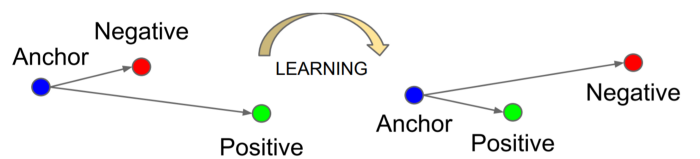
\includegraphics[width=\textwidth]{img/triplet_loss.png}
    \caption[Triplet loss]{The Triplet loss minimizes the distance between an anchor and a positive and maximizes the distance between the anchor and the negative datapoint.\\
    Source: \cite{tripletlossnn}}
    \label{fig:triplet_loss}
\end{figure}

This is the basic idea behind the triplet loss introduced by
\cite{tripletlossfirst} and then further formalized by \cite{tripletlosssecond}
and subsequently used as a loss function for \glspl{nn} by \cite{tripletlossnn}.

We shall use the triplet loss in following form:
\begin{defn}
Triplet loss for selected triplet (A, P, N) is:
\begin{equation}
mathcal{L}(A, P, N) = \text{max}(\delta(f(A), f(P)) - \delta(f(A), f(N)) + \alpha, 0)
\label{eq:triplet}
\end{equation}
Where $f$ is a corresponding to transformation by given \gls{nn}, $\delta$
is a selected distance function and $\alpha$ is a priori selected threshold. The
selected triplet is a triplet of specific samples -- $A$ is a generic point
called ``anchor'' point, $P$ is a ``positive'' sample (i.e. sample of the same
cluster as anchor point) and $N$ is a ``negative'' sample (i.e. sample of
different cluster than anchor point).
\end{defn}

Such definition provides the formula of the loss for specific triplet, however
we can easily extend this notion by considering the average loss over selected
triplets.

It can be easily seen that the minimal value of the Triplet Loss is zero.
In order to achieve this optimal value, not only all ``in-between'' clusters
distances have to be greater then ``within'' cluster distances, but they
must be greater by at least a given margin $\alpha$.

\subsection{Triplet Selection}

Additional challenge for using Triplet Loss is to select suitable triplets.
Usually each point in dataset (or more precisely in a subset of the dataset,
called batch) is once selected as an anchor point. Then the task is then to find
the appropriate positive and negative sample for each anchor point.

The related terminology is somewhat ambiguous. For practical purposes we
chose to use the terminology corresponding to the implementation in Tensorflow
framework (\cite{tensorflow}). They operate with two strategies: Hard and Semi
Hard Triplet Loss.

In case of Hard Loss the positive and negative samples are selected ``as hard as
possible''. Meaning that the positive sample is the furthest sample (from the
anchor point) out of all considered samples of the same cluster. The negative
sample on the other hand is the closes sample out of all samples from samples
that are not of the same cluster as the anchor point.

The Semi Hard approach selects such a pair of positive and negative sample
that the negative sample is further away from the anchor point than the 
positive one, but not by the required margin. In terms of \autoref{eq:triplet}
it means that $\delta(f(A), f(P)) < \delta(f(A), f(N))$ and
$\delta(f(A), f(N)) - \delta(f(A), f(P)) < \alpha$.

% \section{Residual Networks}

% \label{sec:resnet}

% Residual networks (commonly referred as just ResNets) is quite popular family
% of \gls{nn} architectures designed especially for processing images. It was
% officially introduced and described by \cite{resnet} and later improved by
% \cite{resnetimp}. This design gained much popularity by proving the empirically
% proving its quality. They won the first places at ILSVRC competition on the
% tasks of ImageNet detection, ImageNet localization (\cite{imagenetresults}) as
% well as COCO detection and COCO segmentation at COCO competition
% (\cite{cocodataset}).

% The authors tried to solve the problem of low training accuracy of the deep
% neural networks compared to their shallower counter parts. This
% counter-intuitive phenomenon led them to following design change.

% For a given layer, instead of learning direct suitable mapping $H(\vec{x})$,
% they designed the layer to learn just the ``residuum''
% $H(\vec{x}) - \vec{x} = F(\vec{x})$ (hence the name). This was achieved by
% adding residual connection between layer $n$ and layer $m > n$.
% The output of layer $n$ and layer $m - 1$ would be added
% together effectively pushing the layer $m$ to learn the residuum with respect to
% the output of layer $n$ rather then the complete golden function.

% The rationale behind this change is that by adding layers that perform identity
% function we can not worsen (or change at all for that matter) the output of the
% network. Therefore, if we take shallow network and increase its complexity by
% adding new layers the (training) error should not decrease if the learning to
% approximate identity function is easily achieved. However, as the training
% error increases in traditional design it can be argued that to learn identity
% function is quite hard using traditional gradient descent algorithm. By adding
% the residual connection the problem of learning to approximate identity function
% became just a task of driving the weights of the connection to zero, which
% should be easier that to learn identity function directly. As already mentioned
% this rationale was successfully empirically tested on several datasets.

% The original authors further improved this design in \cite{resnetimp} by
% reorganizing the layers in the network. They removed the activation function
% from the residual connection (or, more precisely, they moved it to ``skipped''
% part of the \gls{nn}). This way thay simplified the shortcut even more. They
% further support this change by thorough empirical testing.

% \section{MobileNets}

% \label{sec:mobilenet}

% Other notable architecture are MobileNets by \cite{mobilenets}. In this
% architecture the authors provide models with relatively low latency while
% maintaining high level of accuracy. The motivation behind such architecture is
% to provide suitable models for usage in mobile vision application. They
% lower the latency of inference by simplifying the model.

% Most notable change is the replacement of standard convolution layers as
% described in \autoref{sec:conv} by pair of layers -- depthwise convolutional
% filter and pointwise convolution filter.

% In the first of these layers -- depthwise convolutional filter -- the convolution is applied on each input channel
% separately:
% $$y_{i, j, r} = \sum_{k, l} x_{i+k, j+l, r} c_{i, j, r}$$
% The latter of these two layers -- pointwise convolution filter -- is just simple convolution with kernel of size
% $1 \times 1$.

% This replacement of the convolutional layer by two simpler layers significantly decreases the computation cost of inference, as well
% as the time required for training such network. Furthermore the accuracy of
% resulting \glspl{nn} was verified on the ImageNet task.

% This architecture was then further improved by \cite{mobilenetv2} by
% introduction of inverted residuals and linear bottlenecks. As these concepts
% are quite complex we refer the reader to the original article for more
% information.